
\chapter{Analyzer System}

Total implementation link for data analyzer : \\
\url{https://github.com/Sprea22/Python_Systems}

During this part the main purpose is to analyze the whole dataset in order to find some kind of useful informations later on. 

The system that it's going to be implemented during this part of the work could be divided in two subsystems, with the relative outcomes:
\begin{itemize}
\item Single Input Analyzer (SIA): Used for analyze a single data input.
\begin{itemize}
\item Total graphic of the input data for the whole period.
\item Graphic of the input data for each single year.
\item Correlation matrix between different months of the same input.
\item Correlation matrix between different years of the same input.
\end{itemize}
\item Multiple Inputs Analyzer (MIA): Used for analyze multiple data inputs.
\begin{itemize}
\item General correlation matrix between all the different inputs.

\item Graphic of the normalized angular coefficients of all the inputs.
\end{itemize}
\end{itemize}

\newpage

\section{Requirements for reusability}
Both the analysis systems that are going to be implemented during this phase of the work will need for just one requirement about the input dataset:
\begin{itemize}
\item Monthly frequency of data values.
\end{itemize}

\section{System requirements}
It's important to remind that this phase can be implemented in different ways and with different programming language;\\
This proceure will describes the system implentation using Python, so be sure to have installed all the necessary for compile and execute Python code on your platform.\\
\begin{lstlisting}
Current development environment:
Python version: 2.7.12
Linux kernel version number: Linux Asus 4.4.0-71-generic SMP
\end{lstlisting}

\newpage

\section{Single Input Analyzer}
It's possible to check out the total implementation code of the SIA in the appendice  [\ref{SIA_Implementation}].
The implementation of this Analyzer can be divided in the following parts:
\begin{itemize}
\item SIA imported libraries. 
\item SIA part I: Generate and display a graphic about current input with total data.
\item SIA part II: Generate and display a graphic about current input for each year.
\item SIA part III: Generate and display a graphic that contains the correlation matrix between each single year of the current input.
\item SIA part IV: Generate and display a graphic that contains the correlation matrix between each single months of the year of the current input.
\item SIA part V: Generate and display a single overview image for the current input.
\end{itemize}

\subsection{SIA: Imported libraries}
Specific Python libraries have been imported for the implementation of this system.
It's possible to find out a list of this libraries with a specific description for each of them in the appendice [\ref{SIA_libraries}].

\newpage

\subsection{SIA section I: Total graphic for all the years}
\textbf{Goal:}\\
Generate and display the total graphic about current input, and then calculate and display the trend line as well. Trend line angular coefficient has to be save in a document.

\textbf{Requirements:}\\
The current data input has to be with a monthly frequency. 

\textbf{Implementation:}\\
To reach the current goal have been used two main functions of the "pandas" library. They allow to read the data values from the dataset and display it on a graphic.
\begin{lstlisting}
series = pandas.read_csv()
seris.plot()
\end{lstlisting}

It's possible to check out the full commented implementation in the appendice: [\ref{SIA_section_I}]

\textbf{Results:} \\
With this first part of the code has been reached the first goal of displaying and saving the basic graphic about the current input, with also the relative trend line and saving it angular coefficient in a document, that looks like:

\begin{figure}[H]
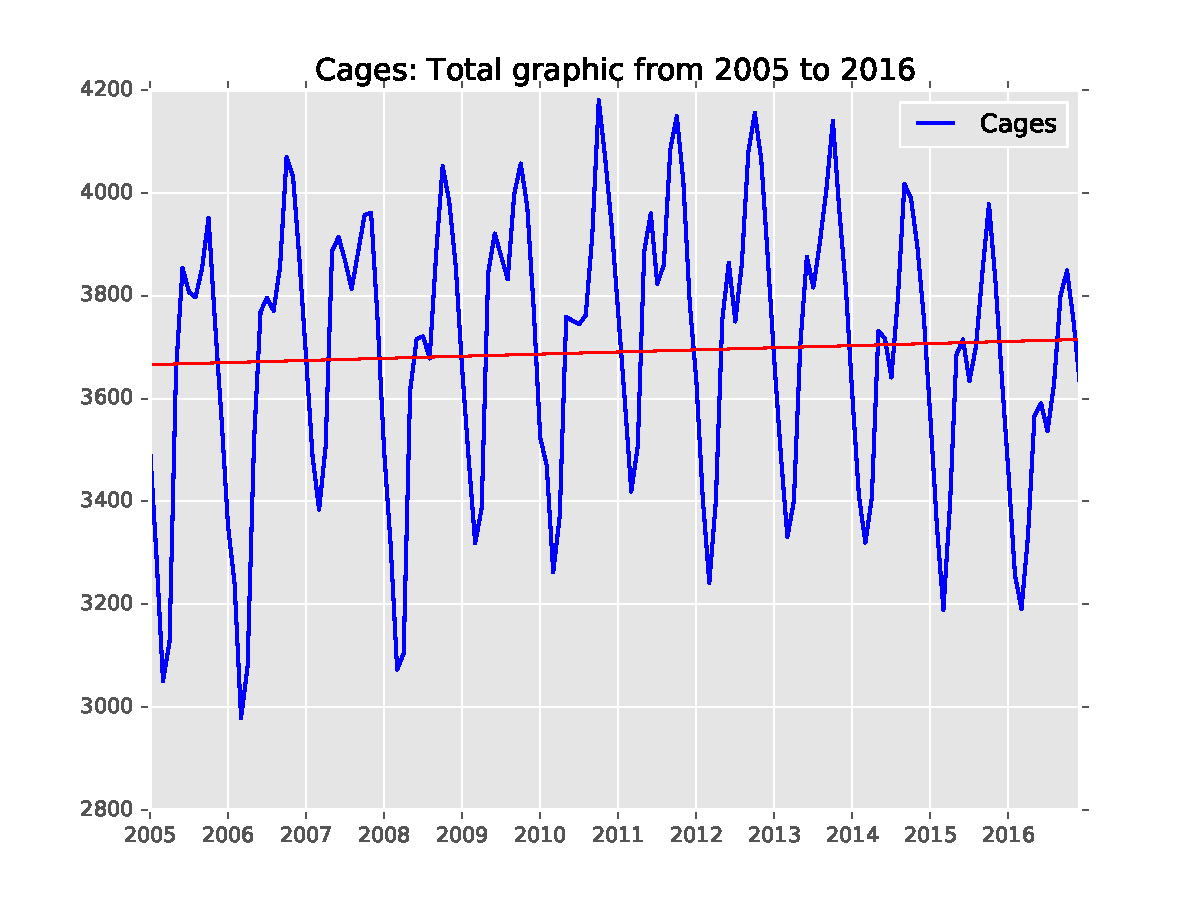
\includegraphics[width=0.9\textwidth]{Files/Cages_Total.pdf}
\caption{Total graphic about current input over the whole period.}
\end{figure}



\newpage
\subsection{SIA section II: Single graphics for each year}

\textbf{Goal:}\\
Generate and display a graphic that contains the plots of each single year over the whole period of the current input. 

\textbf{Requirements:}\\
The current data input has to be with a monthly frequency. 

\textbf{Implementation:}\\
To reach the current goal have been used two main libraries.\\
The "pandas" library allows to read the data values from the dataset and return it like "ndarray" type, then the library "pyplot" allows to display it on a graphic.
\begin{lstlisting}
series = pandas.read_csv()
series.values()
pyplot.plot()
\end{lstlisting}

It's possible to check out the full ccommented code in the appendice: [\ref{SIA_section_II}]

\textbf{Results:} \\
With this second part of the code has been reached the goal of displaying and saving the graphic of the plots for each single year of the current input, that looks like:
\begin{figure}[H]
	\centering
    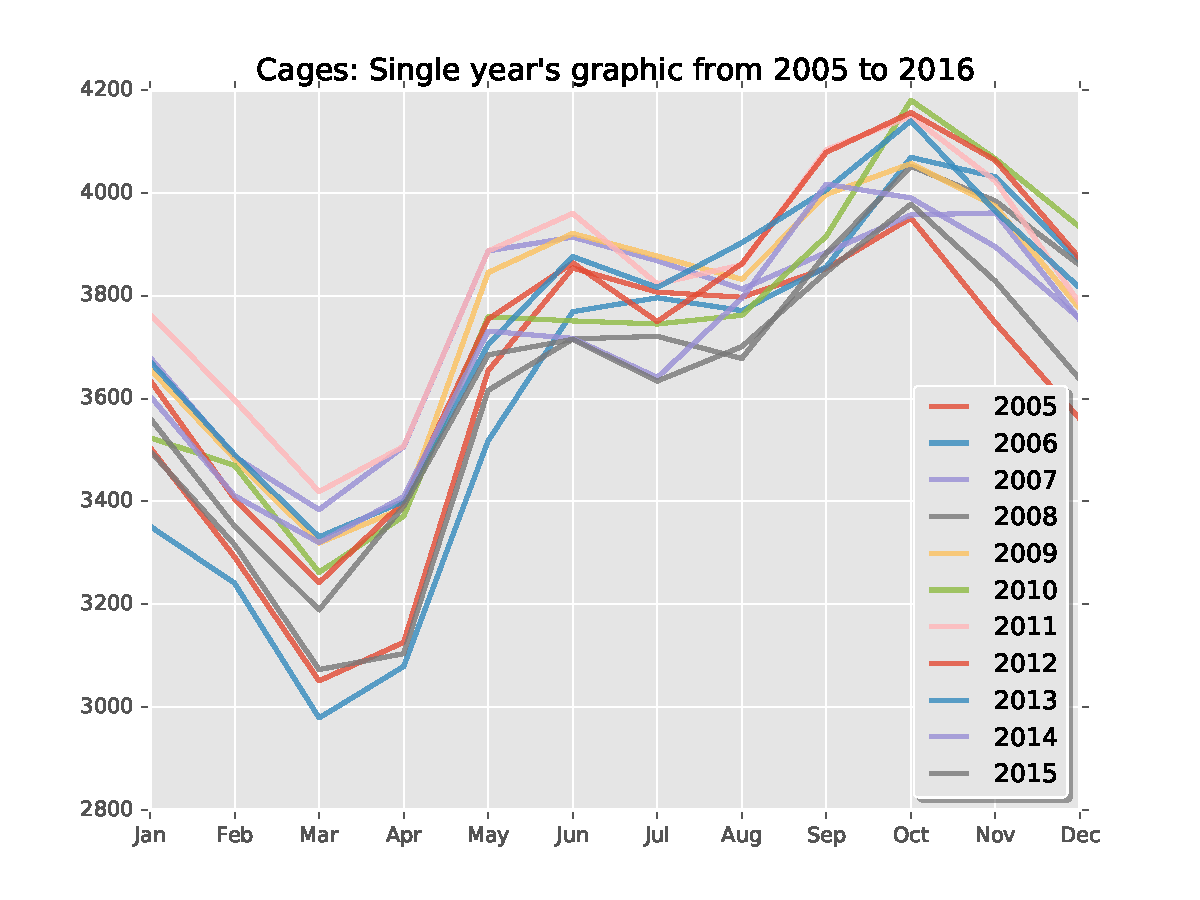
\includegraphics[width=0.9\textwidth]{Files/Cages_Years.pdf}
    \caption{Graphics for each single year of the current input data.}
\end{figure}




\newpage
\subsection{SIA section III: Correlation matrix between years}

\textbf{Goal:}\\
Calculate and save the correlation coefficients between each single year over the whole period of the current input and then display it with a correlation matrix.

\textbf{Requirements:}\\
The current data input has to be with a monthly frequency. 

\textbf{Implementation:}\\
To reach the current goal have been used the scientific computing library "numpy", that allows to calculate the correlation coefficients between data. Then the library "pyplot" has been used to display the results on a matrix.
\begin{lstlisting}
numpy.corrcoef()
figure = pyplot.figure()
ax = figure.add_subplot()
ax.matshow()
\end{lstlisting}

It's possible to check out the full ccommented code in the appendice: [\ref{SIA_section_III}]

\textbf{Results:} \\
With this part of the code have been calculated and displayed the correlation coefficients between each single year of the current input, that looks like:

\begin{figure}[H]
	\centering
    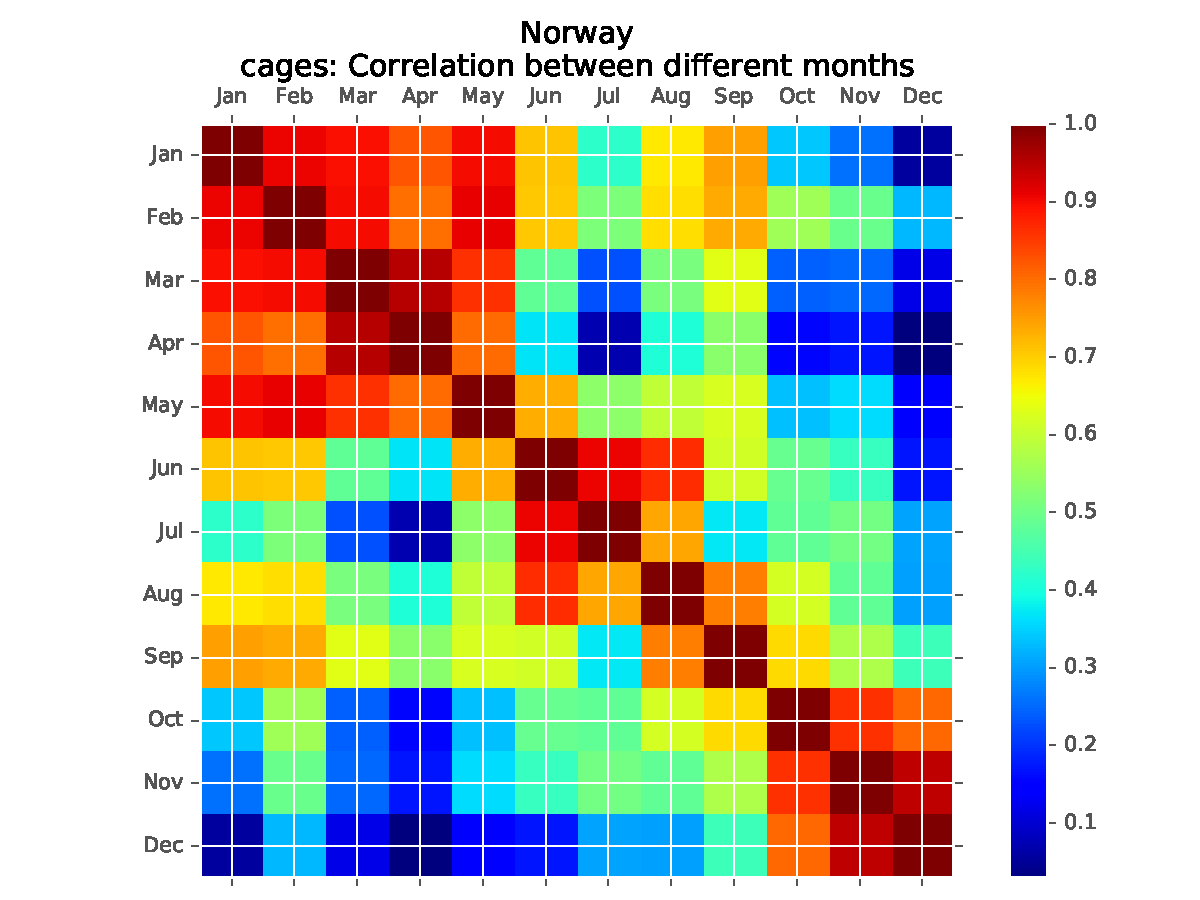
\includegraphics[width=0.9\textwidth]{Files/Cages_Months_Matrix.pdf}
    \caption{Correlation matrix between different months of the same input}
\end{figure}




\newpage
\subsection{SIA section IV: Correlation matrix between months}

\textbf{Goal:}\\
Calculate and save the correlation coefficients between each single month of the current input and then display it with a correlation matrix.

\textbf{Requirements:}\\
The current data input has to be with a monthly frequency. 

\textbf{Implementation:}\\
To reach the current goal have been used the scientific computing library "numpy", that allows to calculate the correlation coefficients between data. Then the library "pyplot" has been used to display the results on a matrix.

\begin{lstlisting}
numpy.corrcoef()
figure = pyplot.figure()
ax = figure.add_subplot()
ax.matshow()
\end{lstlisting}

It's possible to check out the full ccommented code in the appendice: [\ref{SIA_section_IV}]


\textbf{Results:} \\
With this part of the code have been calculated and displayed the correlation coefficients between each single month of the current input, that looks like: 

\begin{figure}[H]
	\centering
    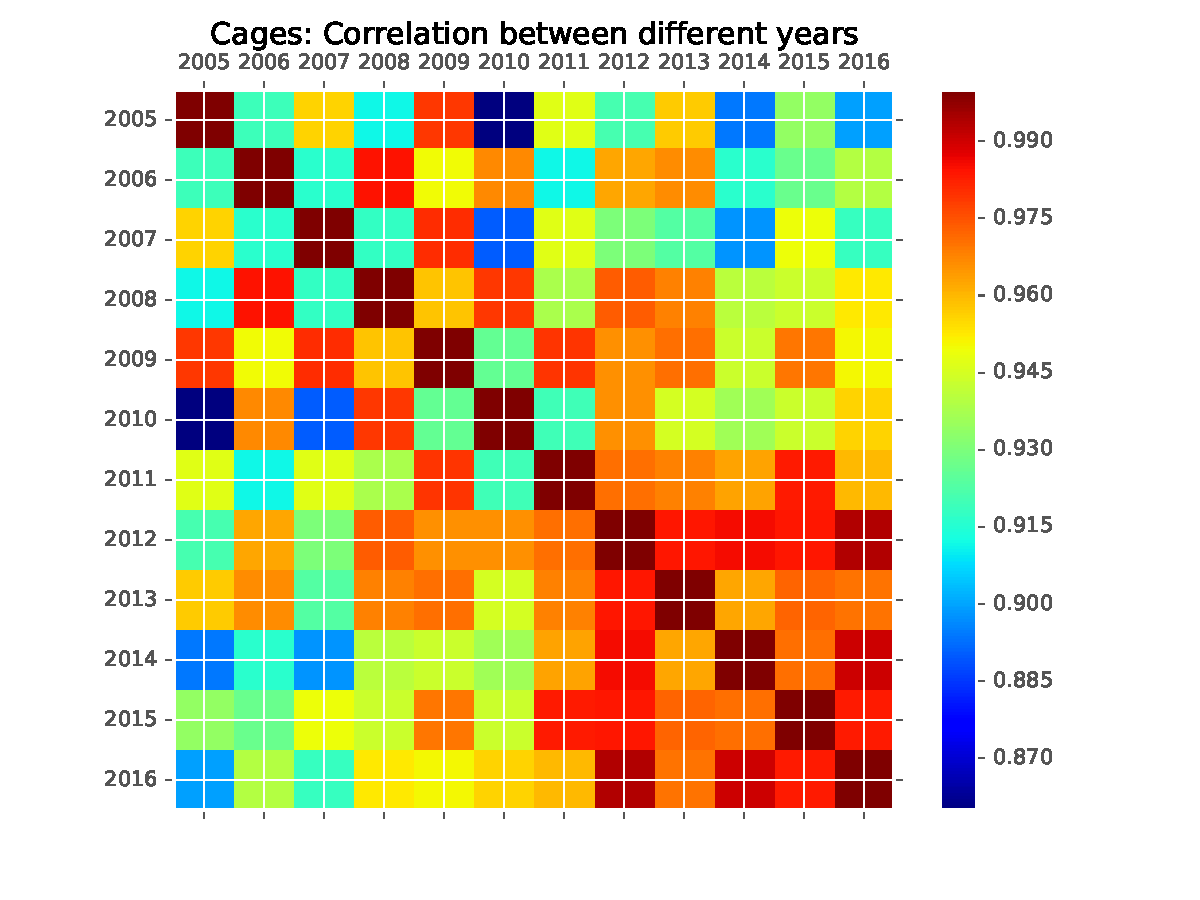
\includegraphics[width=0.9\textwidth]{Files/Cages_Years_Matrix.pdf}
    \caption{Correlation matrix between different years of the same input}
\end{figure}


\newpage
\subsection{SIA section V: Single overview}

\textbf{Goal:}\\
Generate and display a single overview image that contains all the graphics previous calculated about the current input.

\textbf{Requirements:}\\
All the graphics about the current input have to be already calculated and saved.

\textbf{Implementation:}\\
During this part of the implemented system has been indispensable the Python Imaging Library, called also PIL. 
\begin{lstlisting}
from PIL import Image
\end{lstlisting}

It basically allowed to create a new "empty" image and then create a sort of collage pasting the already calculated graphic's images on it.
\begin{lstlisting}
new_im = Image.new()
new_im.paste()
\end{lstlisting}

The following method contains the full code that allows to create the overview image. 
\begin{lstlisting}
def create_single_overview(cols, rows, dest, width, height, listofimages):
\end{lstlisting}
The output of this phase depends by the input to this method, that are basically the list of image and the preferences about the collage's structure.\\
Is possible to view the final result of this phase in the next page and is possible to check out the full ccommented code in the appendice: [\ref{SIA_section_V}]

\newpage

\textbf{Results:}\\
With this part of the code it's possible to have a single overview image about the current input, that basically allows to compare all the graphics already calculated about this input. The general overview graphic contains:
\begin{itemize}
\item Total graphic of the input data for the whole period.
\item Graphic of the input data for each single year.
\item Correlation matrix between different months of the same input.
\item Correlation matrix between different years of the same input.
\end{itemize}

\begin{figure}[H]
\begin{subfigure}{.5\textwidth}
	\centering
    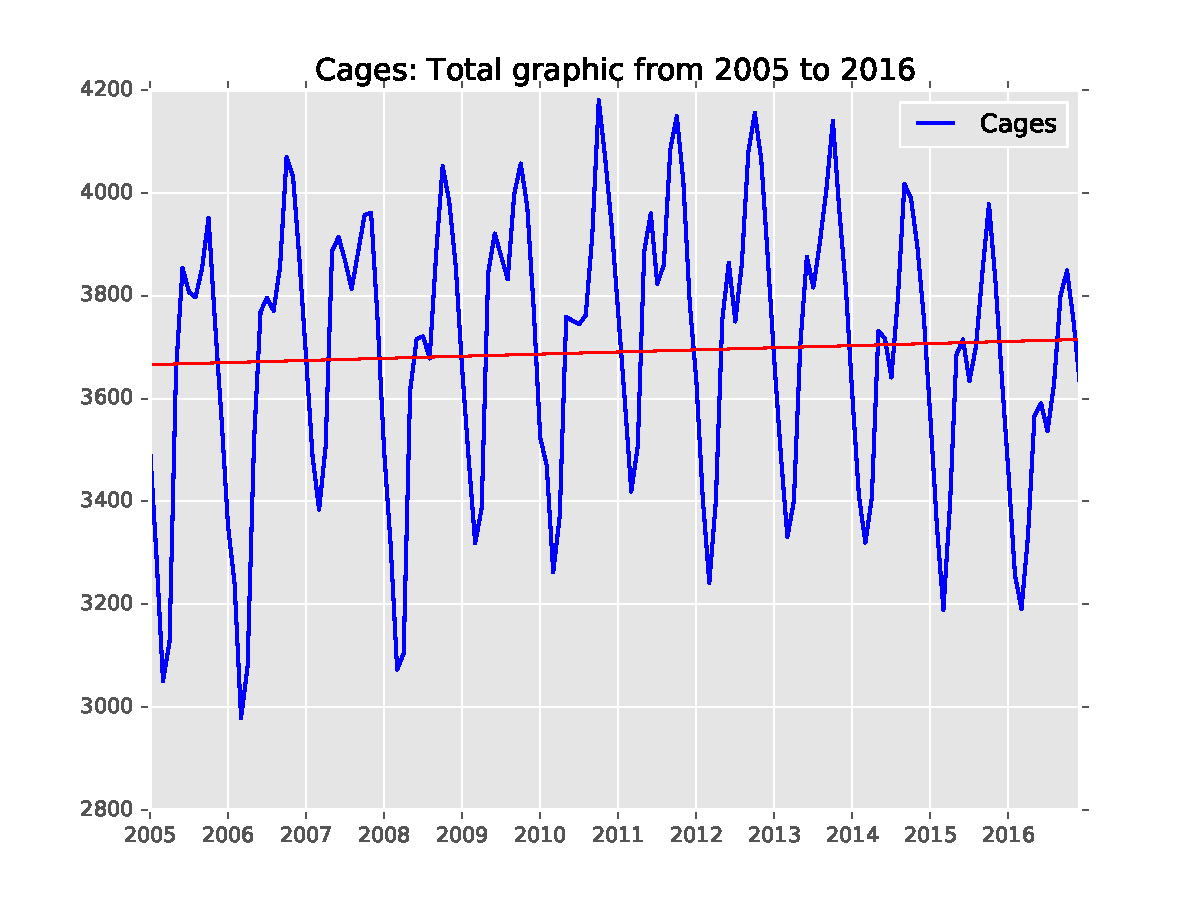
\includegraphics[width=1\textwidth]{Files/Cages_Total.pdf}
\end{subfigure}%
\begin{subfigure}{.5\textwidth}
	\centering
    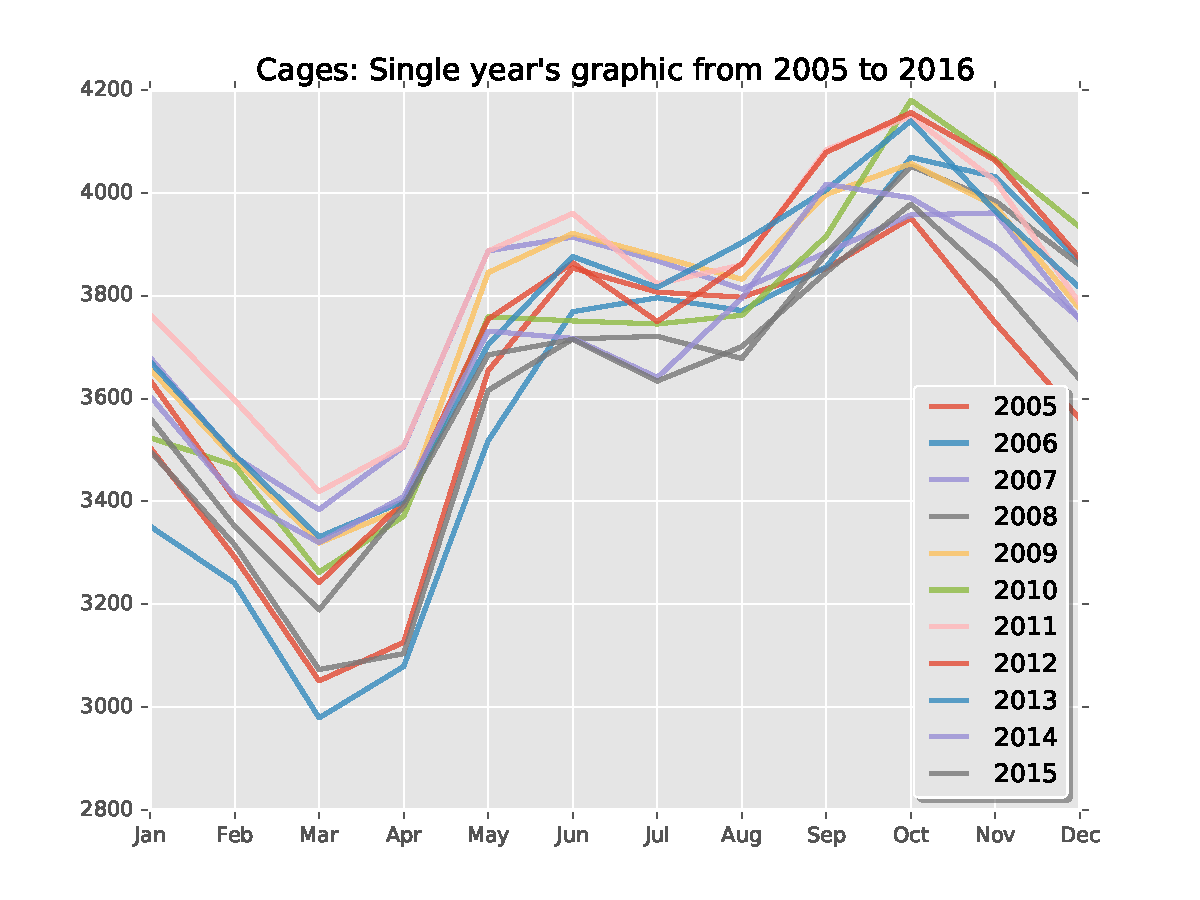
\includegraphics[width=1\textwidth]{Files/Cages_Years.pdf}
\end{subfigure}%
\end{figure} 

\begin{figure}[H]
\begin{subfigure}{.5\textwidth}
	\centering
    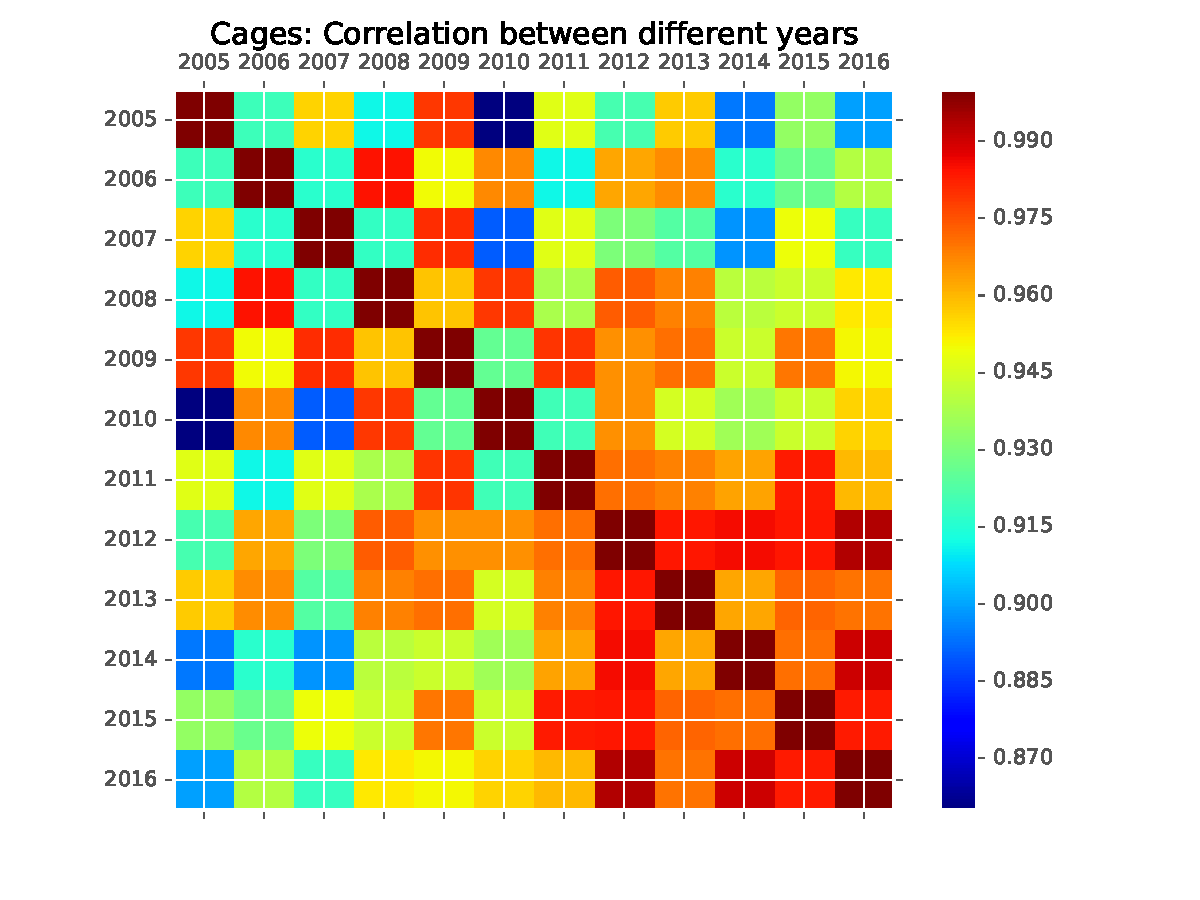
\includegraphics[width=1\textwidth]{Files/Cages_Years_Matrix.pdf}
\end{subfigure}%
\begin{subfigure}{.5\textwidth}
	\centering
    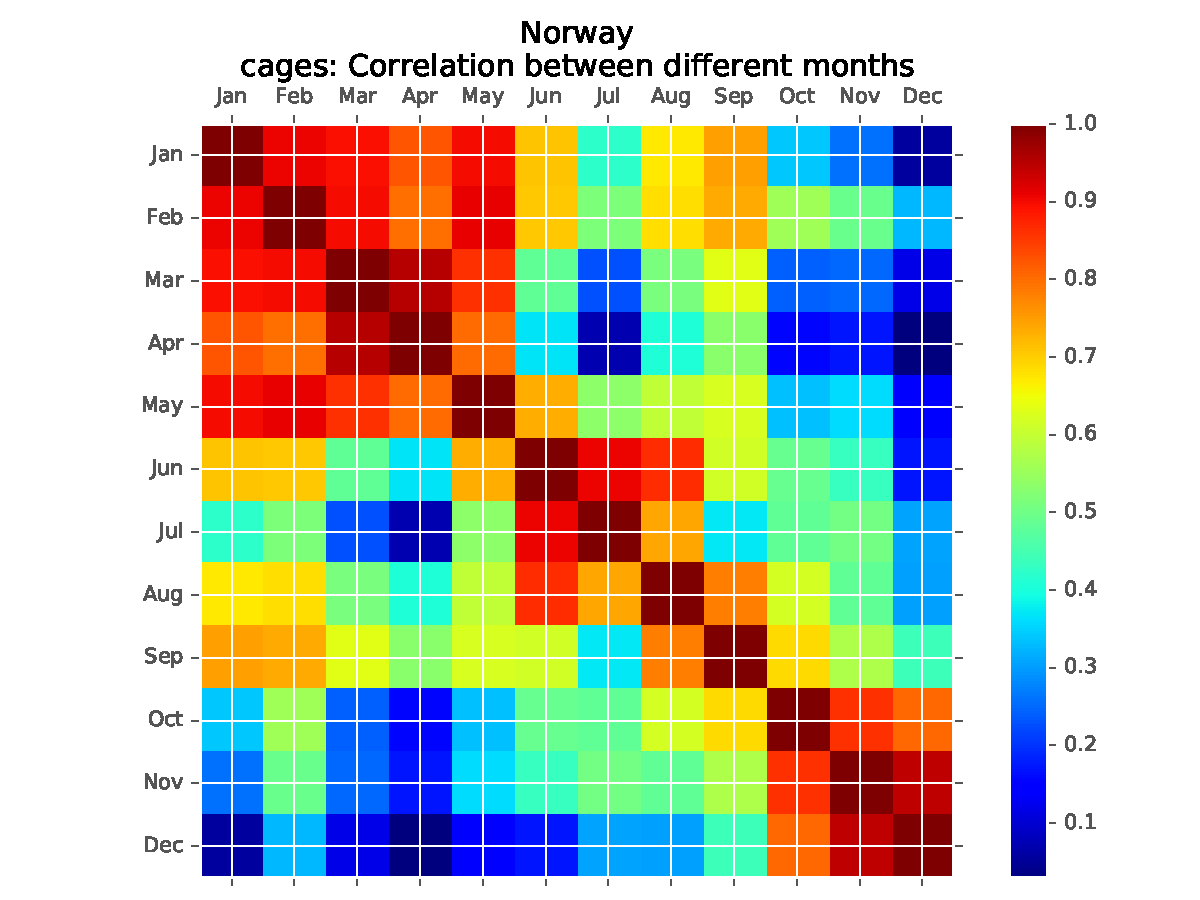
\includegraphics[width=1\textwidth]{Files/Cages_Months_Matrix.pdf}
\end{subfigure}%
\end{figure}

\newpage

\section{Multiple Inputs Analyzer}
The implementation of this Analyzer can be divided in the following parts:
\begin{itemize}
\item MIA imported libraries. 
\item MIA part I: Calculate the correlation coefficients between the different input of a dataset, save the result and display it in a matrix.
\item MIA part II: Display the comparison graphic between the different input's trend line normalized angular coefficients.
\end{itemize}

It's possible to check out the total implementation of the MIA in the appendice  [\ref{MIA_Implementation}].

\subsection{MIA: Imported libraries}
Specific Python libraries have been imported for the implementation of this system.
It's possible to find out a list of this libraries with a specific description for each of them in the appendice [\ref{MIA_Libraries}].

\newpage

\subsection{MIA section I: Total Correlation Coefficients}
\textbf{Goal:}\\
Calculate and save the correlation coefficients between different inputs of the current dataset and then show it with a matrix.

\textbf{Requirements:}\\
To let the MIA system works in a proper way, is necessary that the current dataset has been already analyzed from the SIA system.

\textbf{Implementation:}\\
To reach the current goal have been used the scientific computing library "numpy", that allows to calculate the correlation coefficients between data. Then the library "pyplot" has been used to display the results on a matrix.
\begin{lstlisting}
numpy.corrcoef()
figure = pyplot.figure()
ax = figure.add_subplot()
ax.matshow()
\end{lstlisting}

It's possible to check out the full ccommented code in the appendice: [\ref{MIA_section_I}]

\textbf{Results:} \\
This part of the MIA implementation allows to calculate the correlation coefficients value between each single inputs and then also to display and save it. It looks like:

\begin{figure}[H]
	\centering
    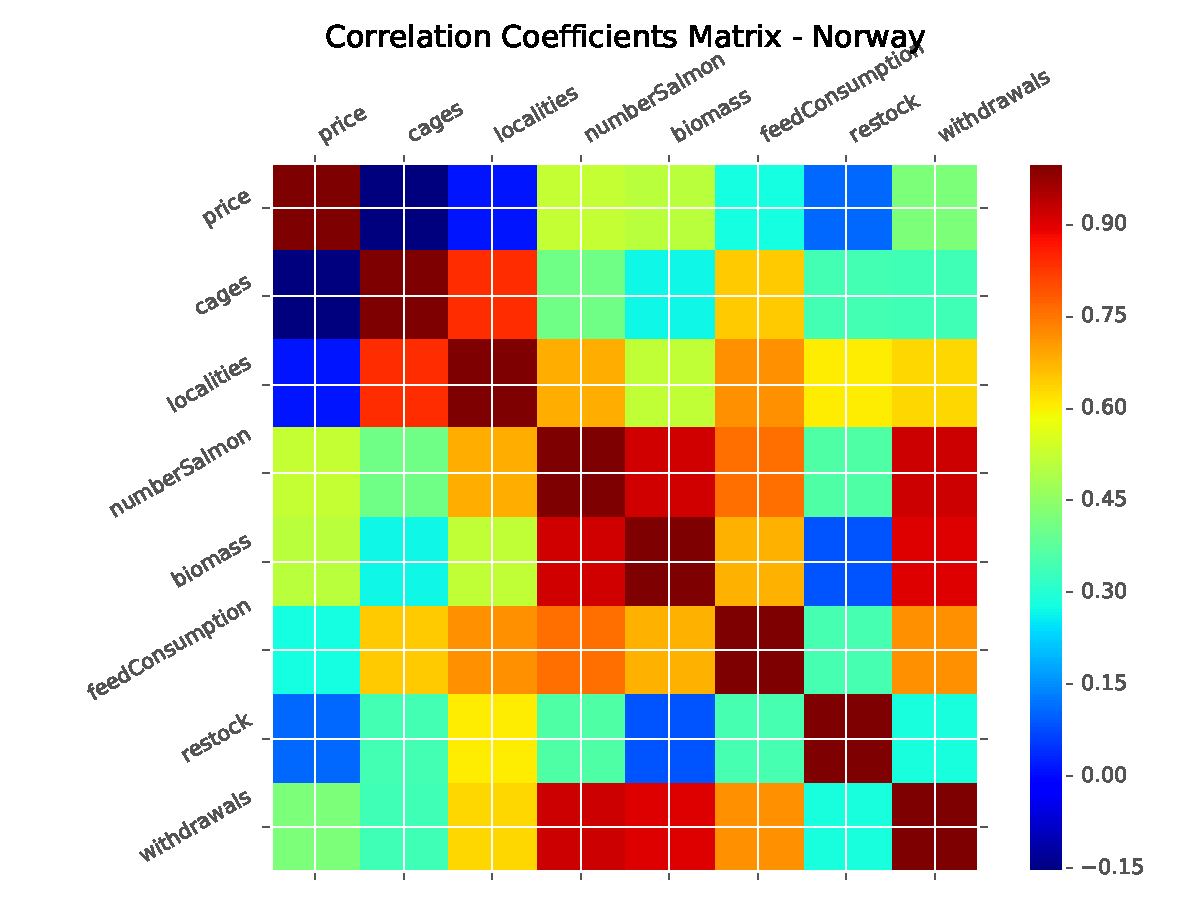
\includegraphics[width=0.85\textwidth]{Files/Total_Dataset_Matrix.pdf}
    \caption{Correlation matrix between different inputs with data.}
\end{figure}

\subsection{MIA section II: Normalized Angular Coefficients}
\textbf{Goal:}\\
Display the comparison graphic between the normalized angular coefficient of each input trend line.

\textbf{Requirements:}\\
To let the MIA system works in a proper way, is necessary that the current dataset has been already analyzed from the SIA system.

\textbf{Implementation:}\\
Also to reach this goal have been used the two libraries "pandas" and "pyplot". The first one allows us to read the values that the library "pyplot" will display, in this case in a histogram.
\begin{lstlisting}
pandas.read_csv()
pyplot.barh()
\end{lstlisting}

It's possible to check out the full ccommented code in the appendice: [\ref{MIA_section_II}]

\textbf{Results:} \\
This part of the MIA implementation allows to display a graphic that compare the normalized angular coefficients for each single input that have been already calculated and reported in a document. The result graphic look like:

\begin{figure}[H]
	\centering
    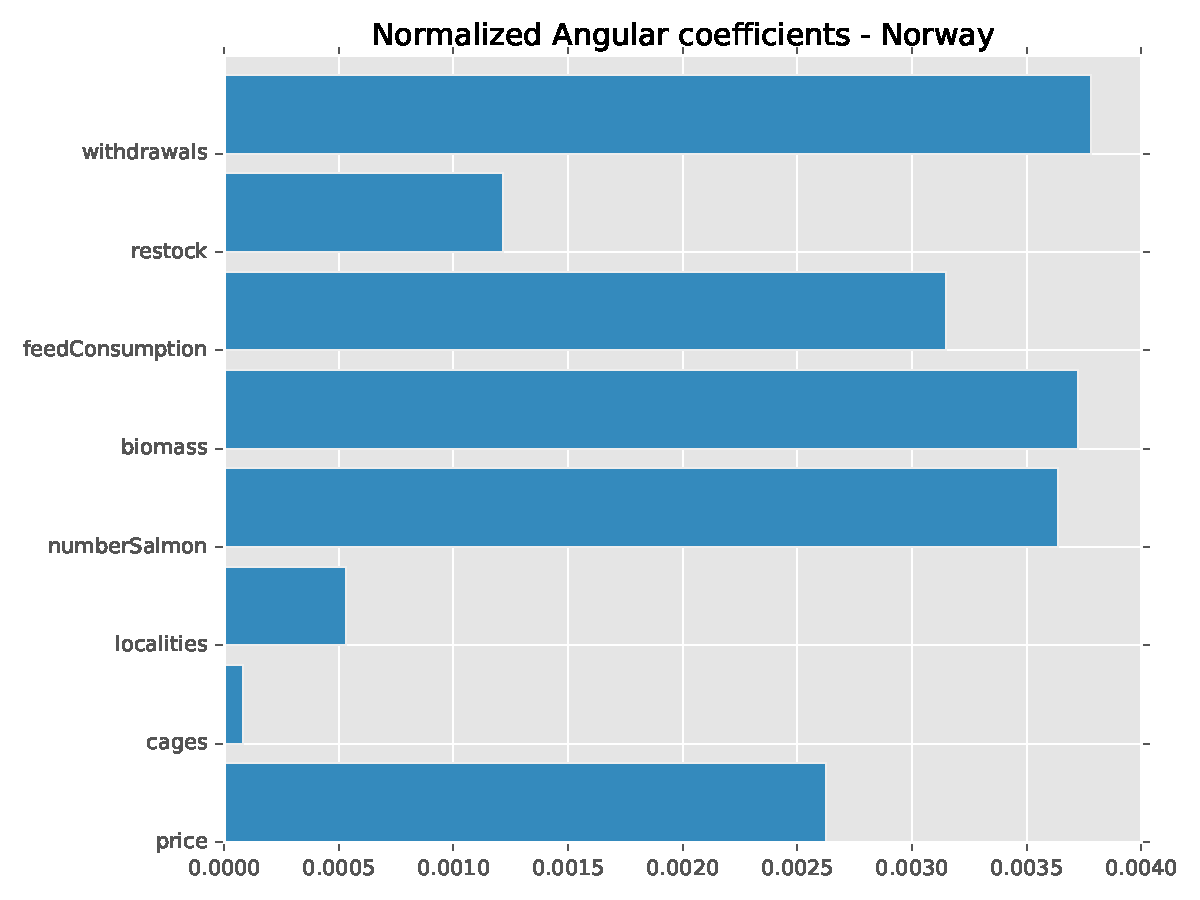
\includegraphics[width=0.90\textwidth]{Files/Norm_Ang_Coeffs.pdf}
    \caption{Normalized angular coefficients of each input's trendline.}
\end{figure}


\newpage

\section{Data Displaying on a map}
\label{Map_displaying}
\textbf{Goal:}\\
The main goal of this phase is to find a way to visualize some data values on a map graphic using Python. In this particular case the map graphic has to represents the Norway territory and its every single county.


\textbf{Requirements:}\\
This displaying system was implemented just for displaying data about Norway, that means it's not reusable for other input datasets.

During this work has been created a specific dataset for test the system works. It contains the average value of a specific input about a single county on the whole available period. The following table shows some examples about the dataset structure: for each county has been calculated the average value from 2007 to 2014 of different parameters.\\

\makebox[\textwidth][c]{
\resizebox{1.2\textwidth}{!}{
    \begin{tabular}{ | l | l | l | l | l | l |}
            \hline
\textbf{county}						&	\textbf{averageSeaTemp}	&	\textbf{cages}				& \textbf{localities}			& \textbf{...}	&  \textbf{feedConsumption/biomass}
	\\ \hline
Finnmark					&	5.2128134819	&	257.2395833333		&	33.8333333333		& ...	& 0.1611964666	\\ \hline
Troms						&	6.2185416667	&	393.3958333333		&	52.1666666667		& ...	&	0.1831404686	\\ \hline
Nordland 					&	6.8333444959	&	804.5104166667		&	109.0208333333		& ...	&	0.1849358645	\\ \hline
Nord-Trondelag				&	7.322600258		&	231.6875			&	30.3645833333		& ...	&	0.1852350478	\\ \hline
Sor-Trondelag				&	7.5381376237	&	306.9479166667		&	51.3645833333		& ...	&	0.1862036956	\\ \hline
More\_og\_Romsdal				&	8.0087820154	&	347.3229166667		&	59.5729166667		& ...	&	0.1831662176	\\ \hline
Sogn\_og\_Fjordane			&	8.1081250683	&	318.9583333333		&	52.5				& ...	&	0.1863151035	\\ \hline
Hordaland					&	7.8033025443	&	738.8854166667		&	131.1770833333		& ...	&	0.1925203347	\\ \hline
Rogaland\_og\_Agder 			&	7.1951075619	&	338.53125			&	53.0416666667		& ...	&	0.1840209916	\\ \hline
    \end{tabular}}}\\
    

\textbf{Implementation:}\\
During the implementation was used the library "cartopy", that provdes cartographic tools for Python. \\
In this particular case has been useful use the library "cartopy.io.shapereader" that allows to read the extension file ".shp", which in this particular case contains the Norway's shape.
\begin{lstlisting}
import cartopy.io.shapereader as shpreader
shpreader.Reader(filename).geometries())
\end{lstlisting}

Then the input shapely geometries were displayed  to the axes using the "matplotlib".
\begin{lstlisting}
plt.figure()
ax = plt.axes()
axes.add_geometries
\end{lstlisting}

Once displayed the geometries on the map, is possible to set their colors based on some input values with the library "matplotlib".
\begin{lstlisting}
plt.get_cmap
matplotlib.colors.Normalize
\end{lstlisting}

It's possible to check out the full ccommented code in the appendice: [\ref{MapNOR}]

\textbf{Results:} \\
During this implementation was implemented a cartographic representation of some parameters about each single county involved in the Norwegian aquaculture business, but is possible to use the reported library to implement a system about an another territory or an another country.
\begin{figure}[H]
    	\makebox[\textwidth][c]{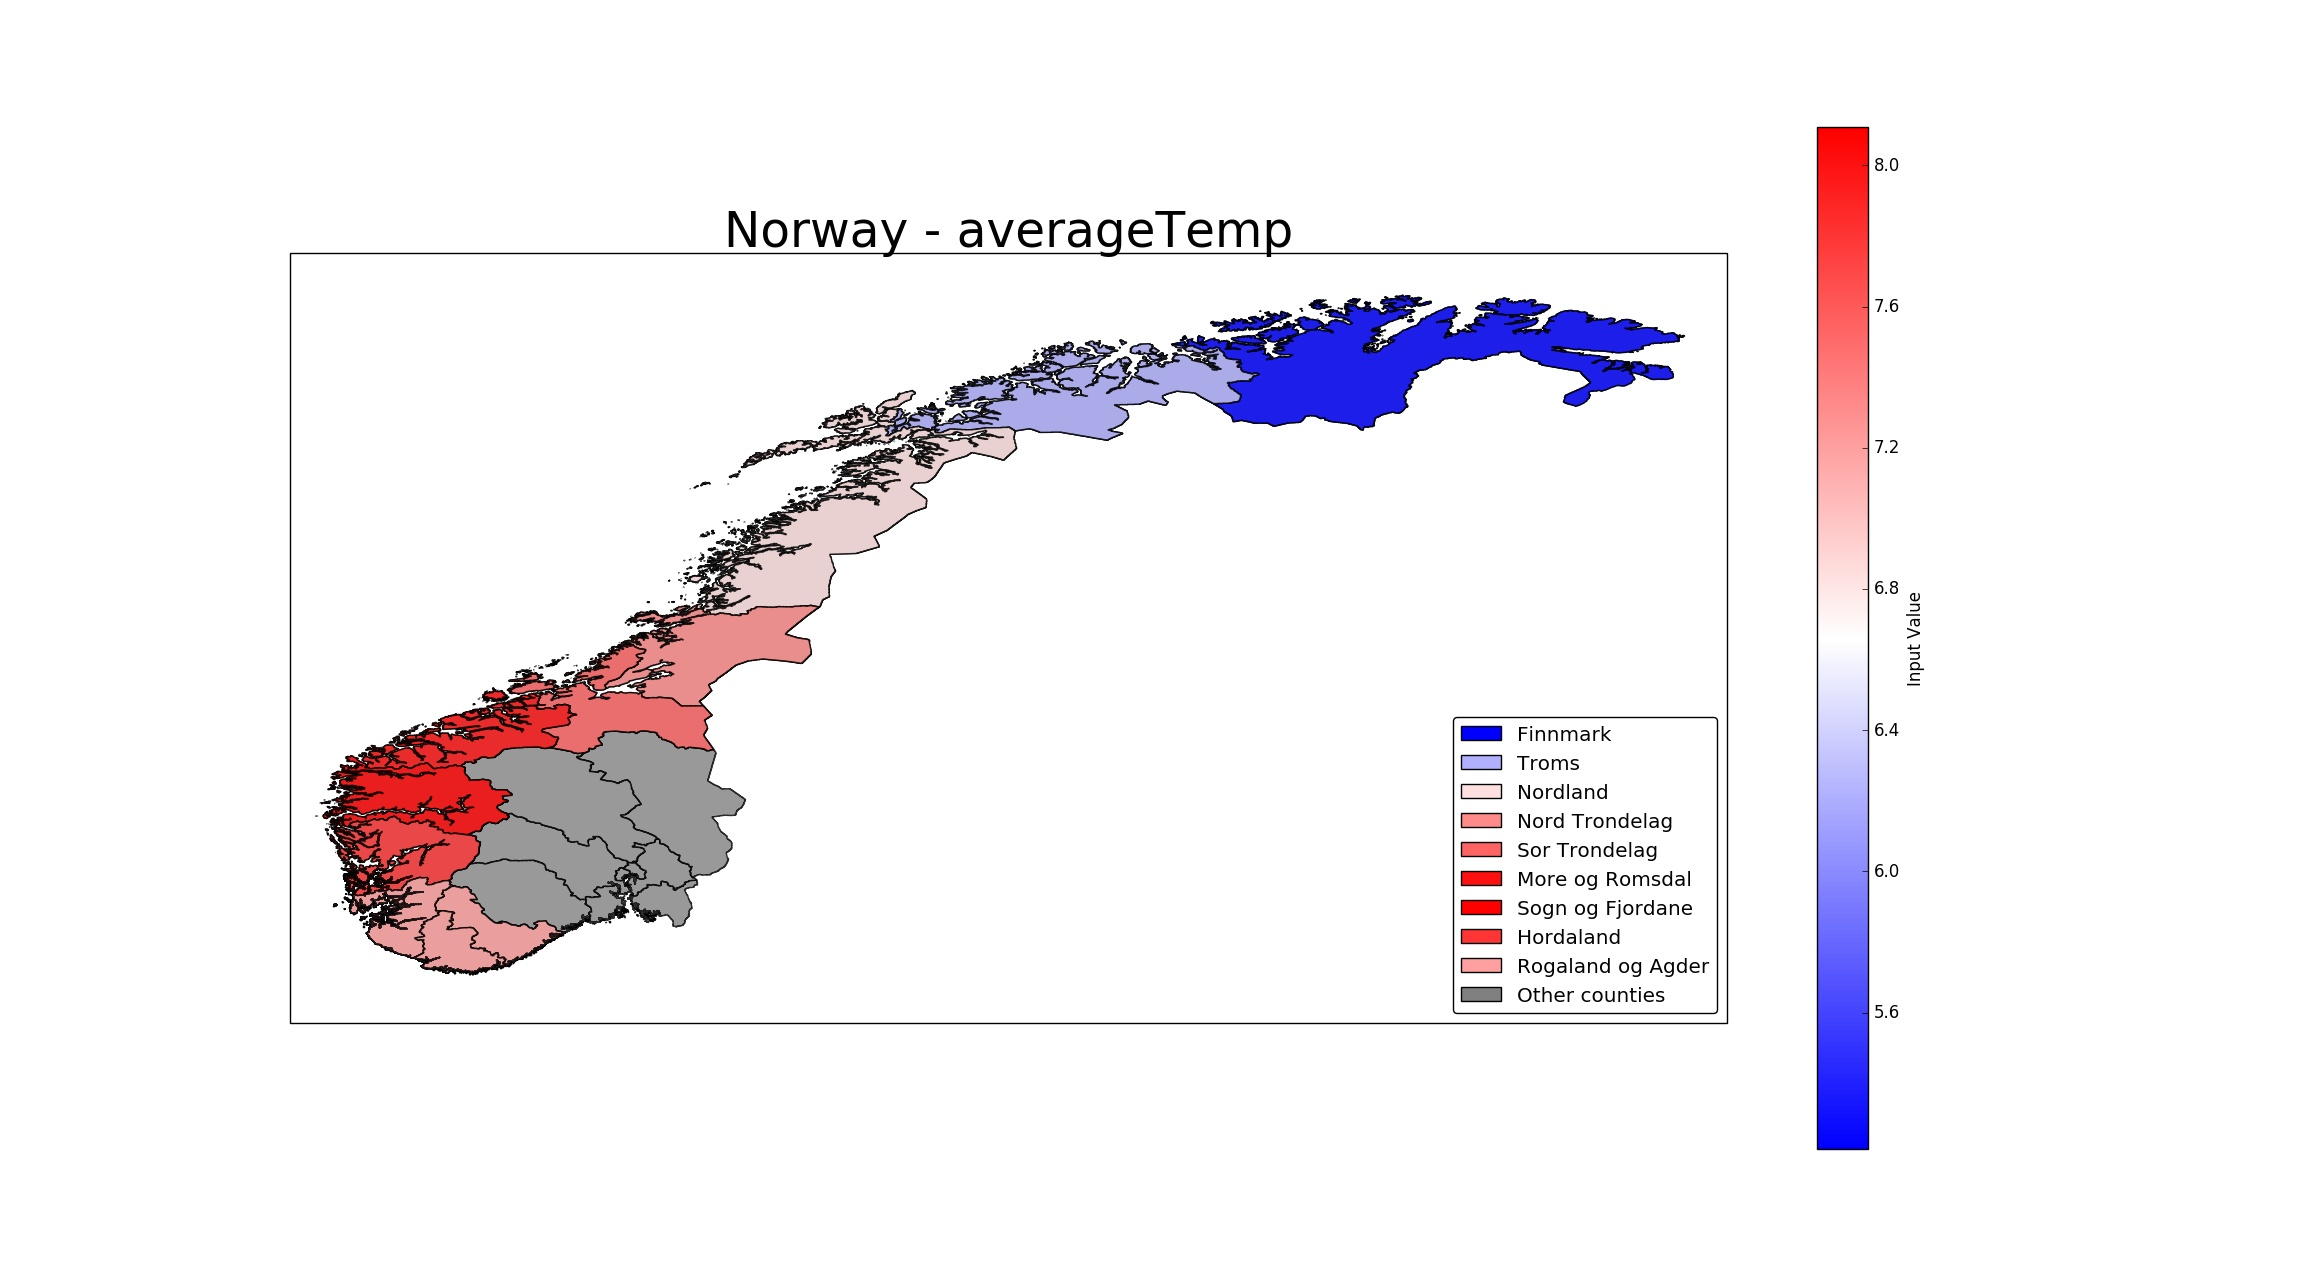
\includegraphics[trim={0cm 2cm 0 3cm},clip, width=1.4\textwidth]{Files/Norway-averageTemp.jpeg}}
    \caption{Average Sea Temperature from 2007 to 2014 in Norway.}
\end{figure}
